\chapter{\textcolor{yellow}{Predicting Stocks Using Sentiment Analysis - Felix}} \label{ch:predictions_ml}
The value of stocks is affected by external events. But information that moves the markets is also captured for example in news articles, online posts on social media or detailed financial reports. One can try to exploit the information presented in the news before it is fully absorbed by the markets. To do so, text data is processed and sentiments are extracted to infer whether the text conveys rather positive or negative information (see \citet{HADDI201326}). Using this information one can either try to predict stocks directly or to forecast future volatility (see \citet{robertson2007news}). This chapter will explore ways to leverage information from news using machine learning to predict the movement of stocks. It will first extract sentiments from text data using two unsupervised learning methods. Secondly, these sentiments will be used for a binary classification of upwards or downwards movement of the ten stocks using XGBoost.

% später
%The news data would need to be as precise as possible, because \citet{gidofalvi2001using} mentions that an effect on the stocks can only be measured up to 20min after the news appear. 
%In a paper by \citet{atkins2018financial} they compare the prediction of stock movement and volatility forecasts using naïve Bayes classifiers. They conclude that movement predictions with 49 Percent accuracy are not successful. 
As we did not have access to good news data, we implemented our approach on the available analyst reports. In contrast to current news, the analyst reports are released much less frequently  and focus more on past performance of stocks than new information. As such they are not able to incorporate current events as quickly as the news. The reports also cluster around certain dates with long stretches of no or very few reports in between (Figure \ref{fig:Seasonality in the Reports}). This makes it unlikely that they are valuable for trading strategies.
\\ 
\section{\textcolor{yellow}{Overview of Existing Methods for Sentiment Extraction}}
There exist several methods to obtain sentiment scores from text data. Most commonly procedures rely on a library of previously known positive and negative words or groups of words called 4-grams. The simplest method, called bag-of-words methods, simply counts the number of positive and negative words in the text. Other approaches extract parts of the text around the location of specific words and then use Support Vector Machines or Naive Bayes Classifier to generate sentiment scores (see \citet{westerski2007sentiment} for further references). Many of these more advanced sentiment classification techniques are supervised learning methods. As such they need a labelled data set for initial training. They are therefore not applicable to our 17153 analyst reports, because these are unstructured and not labelled. Also, the reports have a very specific format and language, therefore other pretrained models or other labelled training data sets could not be used. Other strategies for financial data rely on the availability of intra day trading and news data: By looking at the movement or volatility of the period close after the news release one can estimate approximate sentiment scores \citep{robertson2007news}. As the our stock data is only inter day we could not apply this method.
\\
\section{\textcolor{yellow}{Sentiment Extraction - Theoretical Background}}
Two methods to estimate sentiment scores in an unsupervised way will be explored here. The first one is a library-based approach, the second one is the so called Joint Sentiment Topic Model. 

\subsection{\textcolor{yellow}{Sentiment Library}}\label{BoW}
Our first method for extracting sentiments relies on a library that categorizes words as positive or negative. We can apply this library to the analyst report and obtain the number of positive (P) and the number of negative words (N) in the report. A sentiment or polarity score can then be calculated for each report from the relative frequencies of positive and negative words: 
\begin{equation}
    Polarity = \frac{P - N}{P + N}
\end{equation}
Some more advanced libraries even measure the positiveness of each word with a numeric score (and not only 1 and -1), but we could not find any library appropriate for our purposes. Instead we used a library from \citet{sent_dictionary} as simple word list. An excerpt from the list can be found in table \ref{tab:sent_dic}. 
\begin{table}[ht]
\centering
\begin{tabular}{rll}
  \hline
 & positive & negative \\ 
 & $n = 218$ & $n = 1282$ \\ 
  \hline
  1 & acclaim & abandonment \\ 
  2 & accomplishment & abdication \\ 
  3 & advantage & abuse \\ 
  4 & assure & acquittal \\ 
  5 & attractiveness & catastrophe \\ 
  6 & delightful & criticize \\ 
  7 & diligent & degrade \\ 
  8 & impress & harsh \\ 
  9 & \vdots & \vdots \\ 
   \hline
\end{tabular}
\caption{Excerpt from the sentiment dictionary by 
\citet{sent_dictionary}}
\label{tab:sent_dic}
\end{table}

\subsection{\textcolor{yellow}{Joint Sentiment Topic Model}}\label{JST}

To make the computation of the sentiment scores more adaptable to the specific format of the data, a new method by \citet{lin2009joint}, called Joint Sentiment Topic model (JST), is being used. This approach builds upon the idea of \citet{blei2003latent} to use a Bayesian hierarchical model, called Latent Dirichilet Allocation (LDA), to compute topics from text data. Latend Dirichilet Allocation is one of the most sophisticated methods in the field of topic modelling. To understand JST we firstly explain the fundamentals and assumptions of LDA. \\ 

% good video: https://www.youtube.com/watch?v=DWJYZq_fQ2A
The general idea of LDA is that each document can be described by a distribution of topics and each topic can itself be described by a distribution of words \citep{blei2003latent}. This assumes that the words themselves are independent of each other which is in reality not the case, but for large data sets this assumption seems to be acceptable. To train a LDA one decides on the number of topics ($T$) that occur within the text documents and have not been observed, they are latent. The LDA has two dirichilet priors containing hyperparameters $\alpha$ and $\beta$, a high $\alpha$ indicates that each document is likely to contain a mixture of many topics, similarly a high $\beta$ indicates that each topic is a mixture of many different words. LDA backtracks from the document level to identify topics that are likely to have generated this specific corpus of words. The underlying optimisation of the model is done using a Gibbs-Sampler. In the first step, each word is assigned probabilities to belong to each of the $T$ topics that sum up to one and each document gets a probability for each topic. The algorithm then iterates over the words topics and documents, updating the underlying probabilities. \\ \\
In the JST the LDA is extended from three hierarchical layers to four. The additional layer determines the document sentiment by adding a layer in between the document and topic layer \citep{lin2009joint}. The new sentiment layer can be associated with documents, followed by topics and then words. For a detailed mathematical definition see \citet{lin2009joint}. \\ \\
To estimate the JST models we used the \textit{rJST} package in R \citep{rJST} and added the sentiment dictionary from the previous section \ref{BoW} as prior information for performance improvements.

The output are posterior probabilities for sentiments and topics of each document, as well as the posterior probabilities of each word loading onto topics. For a large and diverse enough training data set the returned posterior probabilities of the words can be used to determine the topics and sentiment in new documents. The JST therefore does not need to be retrained at each new observation. \\





%%%%%%%% Ergebnisse library method %%%%%%%%%%%%

Figure \ref{fig:BoWSentiment} shows the distribution of the sentiment scores we obtained after applying this library method to every single analyst report. The histogram shows an approximate normal distribution around zero. This also means the the imbalance in the number of positive ($n = 218$) and negative ($n = 1282)$) words seems to be about right.
%The results of applying the sentiment library to the reports can be found in figure \ref{fig:BoWSentiment}. The histogram shows an approximate normal distribution around zero. This also means the the imbalance in the number of positive ($n = 218$) and negative ($n = 1282)$) words seems to be about right.
\begin{figure}[h]
\centering
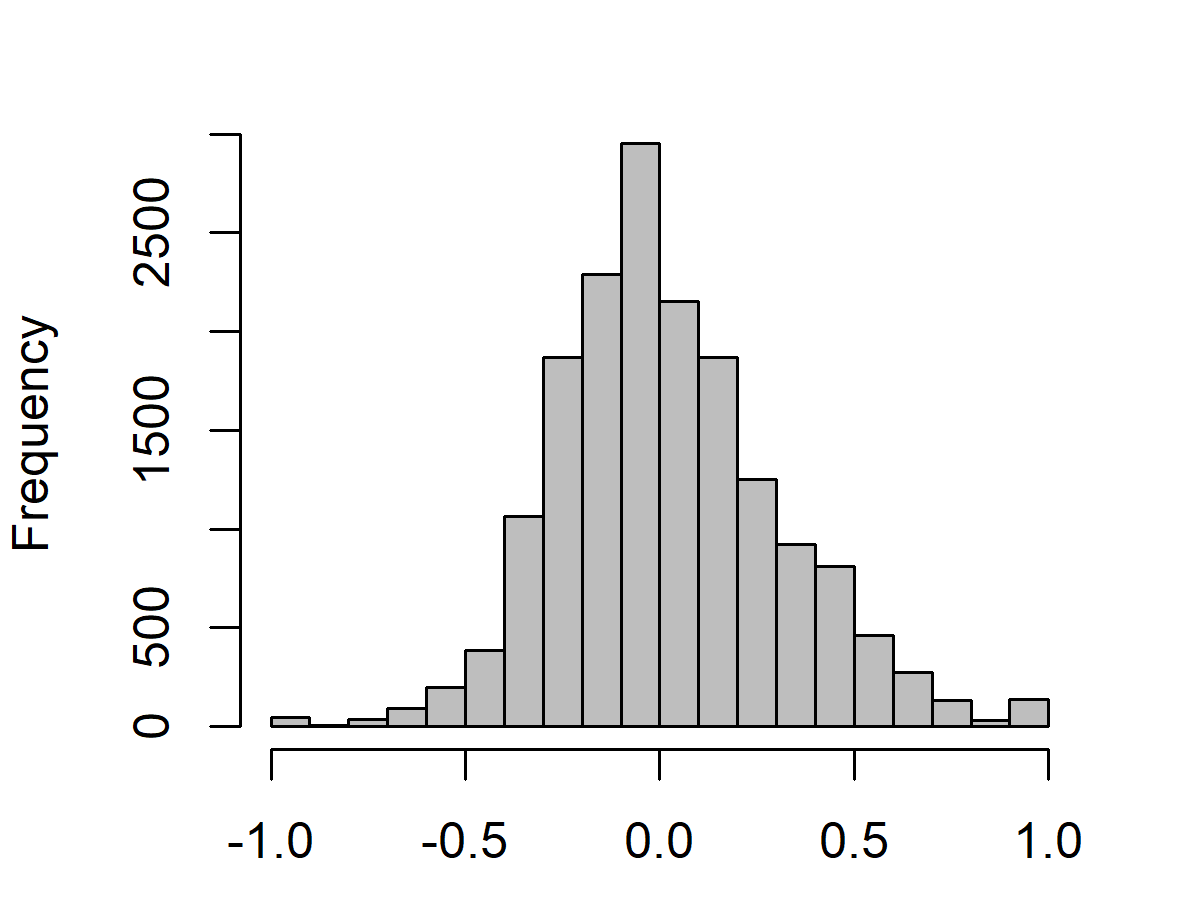
\includegraphics[width=4in]{figures/2SentimentsBOW_Histogram.png}
\caption{Histogram of the sentiment scores computed by the sentiment library}
\label{fig:BoWSentiment}
\end{figure}

One is a library bag-of-words approach that works with simple relative frequencies of positive and negative words. The other approach uses a  method called Joint Sentiment Topic model (JST) \citep{lin2009joint} and relies on a Bayesian method called Latent Dirichilet Allocation (LDA)  \citep{blei2003latent}. For both approaches the text data has to be cleaned which is described in section \ref{cleaningText}, the subsequent analysis of the sentiment scores can be found in section \ref{BoW} and \ref{JST}.

\section{\textcolor{yellow}{Cleaning of the text data}}\label{cleaningText}
The entire set of analyst reports contains 157380 unique words, characters and symbols. Many of them, however, do not really convey meaning or relevant information. To get reliable sentiment scores, the text data therefore has to be cleaned and preprocessed in order to remove noise and reduce the dimensionality of the unsupervised learning problem \citep{HADDI201326}. The preprocessing was done in four steps using \texttt{R} \citep{Rproject} and the \texttt{R} package \texttt{tidytext} \citep{tidytext}. At first, words where converted to lowercase and all words where saved as separate strings. Stop words (like 'the', 'in', 'at') were removed by using a custom stop word library. There exist a lot of readily available stop word libraries, both from the \textit{tidytext} package and from other sources. One problem, however, with many libraries is that they also contain many adjectives that might be important for the extraction of reasonable sentiments. We therefore created our own library of stop words by modifying the existing \texttt{tidytext} stop word library. This first step of removing stop words reduces the total number of words from 67M initially to 43M (see figure \ref{fig:TotWord}). In the second step all special characters, links to websites, hyper-references, numbers, words with numbers and punctuation marks are removed as well. The result reduced the number of unique words and items by about 50 Percent from 157206 to 82525.  \\

\begin{figure}[h]
\centering
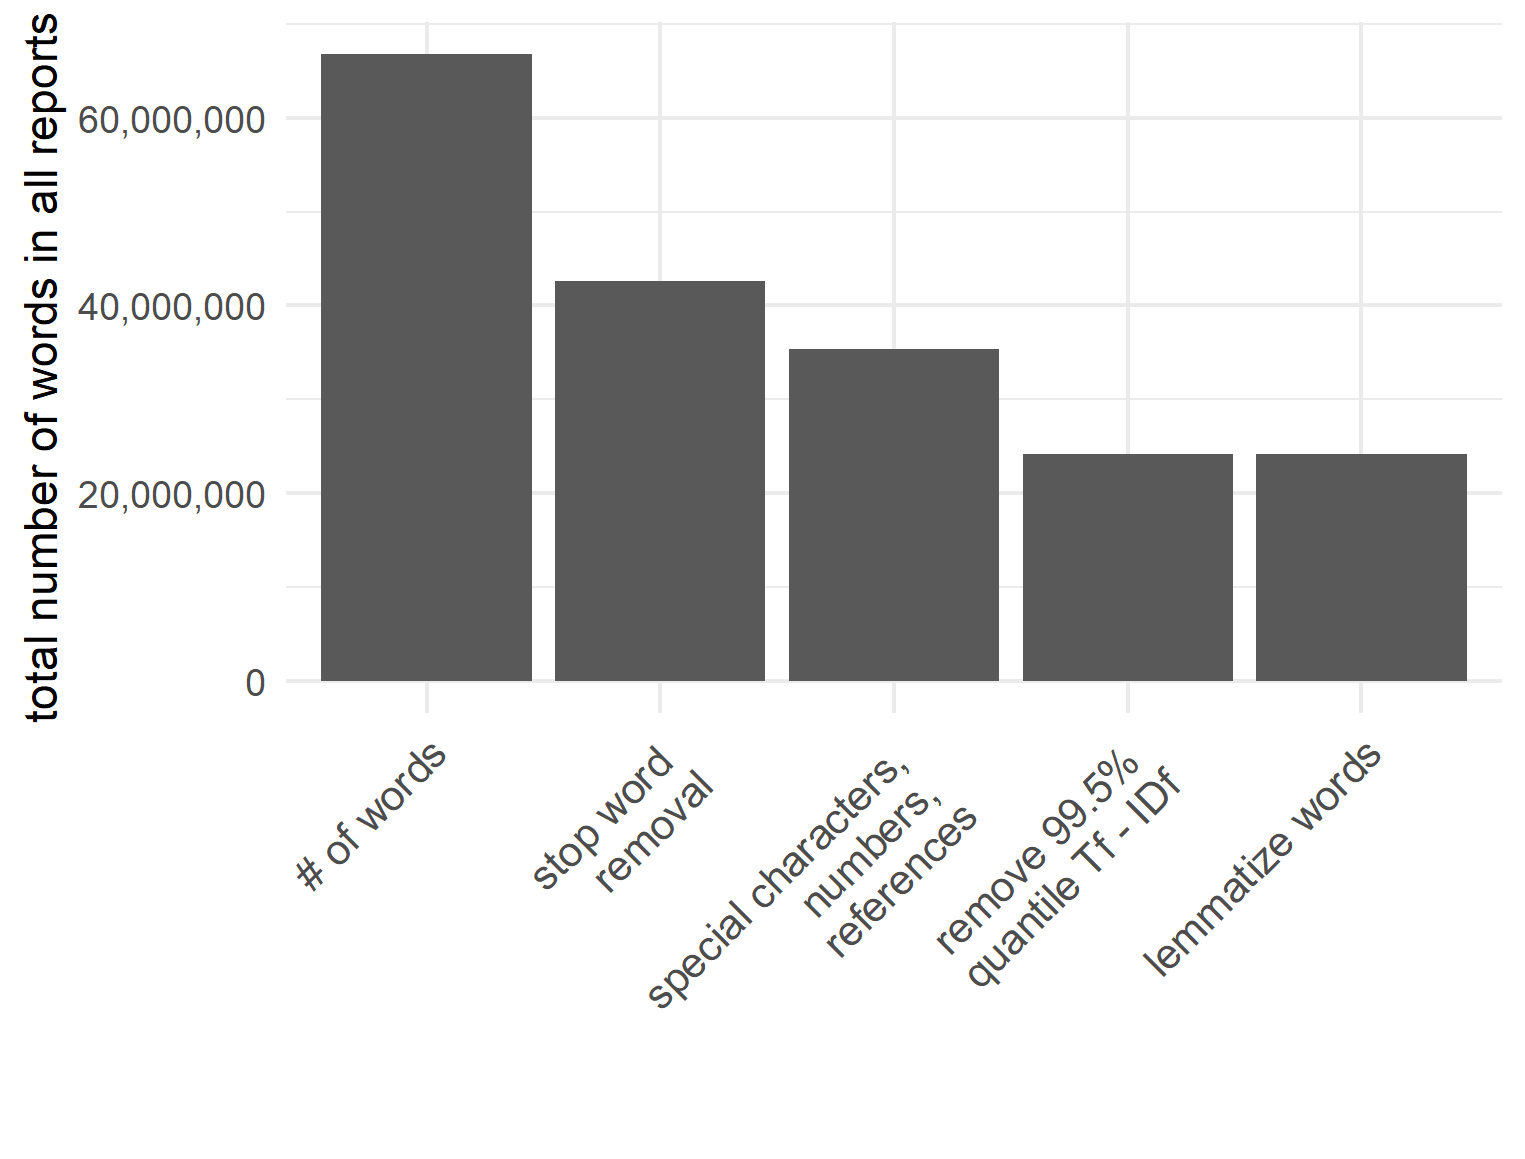
\includegraphics[width=\textwidth]{figures/ReductionInTotalNWords.png}
\caption{Reduction in total number of words due to preprocessing the data.}
\label{fig:TotWord}
\end{figure}

\textcolor{red}{Überleitung, andere Überschrift?}



A common way to look at feature importance in flowing text data is to look at the so called 'Term Frequency Inverse Document Frequency' (TF-IDF) which puts the feature frequency (FF) also called term frequency (TF) in relation to the inverse document frequency (IDF) \citep{na2004effectiveness}. 
\begin{equation}
    TF-IDF = FF * \log{\frac{N}{DF}}
\end{equation} 
Where N represents the number of documents and is DF the number of documents that contain this feature, calculated as the sum of the feature presence (FP). \textcolor{red}{hmm?}
The result is a probability between 0 and 1 for each word. For a large number of words, as in our case, TF-IDF values are usually quite low. For topic modelling like LDA the lower 10 Percent of words are often removed, because they contain relatively frequent words over all documents. Here we are doing the opposite. Due to the structure of the data of ten different stocks and company specific reports we want to avoid fitting company specific topics in the JST model. Removing the 99.5 Percent upper quantile of TF-IDF words seemed to improve the performance. Leaving just over 24M words in total. This represents the removal of an additional 10293 individual words. The fifth and last step is lemmatizing the words using the \textit{textstem} package \citep{textstem}. Lemmatizing words means reducing them to their inflectional forms. We did not stem the words because it sometimes changes the meaning of words, which is important for sentiment analysis. \textcolor{red}{Beispiel vielleicht?}\\ \\


%A common way to look at feature importance in flowing text data is to look at the Term Frequency Inverse Document Frequency (TF-IDF) which puts the feature frequency (FF) also called term frequency (TF) in relation to the inverse document frequency (IDF) \citep{na2004effectiveness}. 
%\begin{equation}
%    TF-IDF = FF * Log(\frac{N}{DF})
%\end{equation} 
%Where N represents the number of documents and is DF the number of documents that contain this feature, calculated as the sum of the feature presence (FP). The result is a probability between 0 and 1 for each word. For a large number of words, as in our case, TF-IDF values are usually quite low. For topic modelling like LDA the lower 10 Percent of words are often removed, because they contain relatively frequent words over all documents. Here we are doing the opposite. Due to the structure of the data of ten different stocks and company specific reports we want to avoid fitting company specific topics in the JST model. Removing the 99.5 Percent upper quantile of TF-IDF words seemed to improve the performance. Leaving just over 24M words in total. This represents the removal of an additional 10293 individual words. The fifth and last step is lemmatizing the words using the \textit{textstem} package \citep{textstem}. Lemmatizing words means reducing them to their inflectional forms. We did not stem the words because it sometimes changes the meaning of words, which is important for sentiment analysis. \\ \\

After these five cleaning steps the number of individual words and items was reduced from 157380 to 64228 by about 60 Percent and of the total number of words only 36 Percent are left. The summary statistics for the total number of words in each report in table \ref{tab:summaryCR} show the result more clearly. 
\begin{table}[ht]
\centering
\begin{tabular}{rllllll}
  \hline
  & Min. & 1st Qu. & Median  &  Mean & 3rd Qu. &   Max. \\
  \hline
  original reports & 16  &  1913  &  3230 &   3834  &  4785  & 21502  \\ 
  cleaned reports  & 0   &  729  &  1232  &  1400  &  1803  &  7218  \\ 
   \hline
\end{tabular}
\caption{Summary statistics for the number of words in each report}
\label{tab:summaryCR}
\end{table}

%After validating the cleaned text different uncleaned items, like words consisting of multiples of the same letter, where discovered. We did not find a way to remove them.

 \\
The results of the JST model need to be evaluated if the results split the data in reasonable topics and associated sentiments. Because we do not have any labelled training data we cannot check the convergence of the model with classical accuracy scores used in \citet{lin2009joint}. Instead we examine the highest loading words per sentiment and topic and the distribution of the sentiment scores. Due to the fact that we only have analyst reports for ten different stocks the results of the JST can at least be questioned. During the training of different models and experimenting with different data preparation steps the model often indicated splitting the data on special stock specific topics, instead of general topics associated with sentiments. Improvements where achieved by using a custom stop word dictionary that only contains few adjectives and the removal of the 99.5 Percent quantile of the TF-IDF words. We decided on using the JST model with 30 topics by comparing the results of models with 10, 20, 30 and 50 topics for different learning rates and numbers of iteration, because it returned the most reliable results. \\

Table \ref{tab:tab:postProbSent1} gives an overview over the words  with the highest posterior probability for sentiment one on topic one to three and thirty (see appendix for Table sentiment two \ref{tab:postProbSent2} ). It is still visible that the documents are from a business context but words indicating the sentiment like good, growth, high are only few. This makes it hard to tell if sentiment one is positive, negative or even something different. \\
% latex table generated in R 3.6.0 by xtable 1.8-4 package
% Fri Sep 13 15:15:05 2019
\begin{table}[ht]
\centering
\begin{tabular}{rllll}
  \hline
 & topic1sent1 & topic2sent1 & topic3sent1 & topic30sent1 \\ 
  \hline
1 & good & year & customer & price \\ 
  2 & look & margin & year & volatility \\ 
  3 & company & will & service & day \\ 
  4 & just & good & will & stock \\ 
  5 & question & growth & business & financial \\ 
  6 & mean & market & believe & average \\ 
  7 & make & expect & continue & expect \\ 
  8 & want & service & datum & year \\ 
  9 & right & continue & growth & next \\ 
  10 & business & high & line & group \\ 
  11 & talk & next & fix & express \\ 
  12 & people & single & also & report \\ 
  13 & time & still & price & month \\ 
  14 & content & also & industry & rate \\ 
  15 & without & digit & time & person \\ 
   \hline
\end{tabular}\label{tab:postProbSent1}
\caption{Words for sentiment one with highest posterior probability per topic}
\end{table}
Another way to evaluate the model is to take a closer look at the posterior probabilities for the sentiments. The histogram in figure \ref{fig:JSTSentiment} displays a reasonable split done by the sentiments. As we computed only positive and negative sentiment scores and left out a neutral class the histogram for sentiment two is this one flipped. The calculated sentiments also seem to lean towards the left. This might indicate that sentiment two was the more prominent one in the data. \\
\begin{figure}[h]
\centering
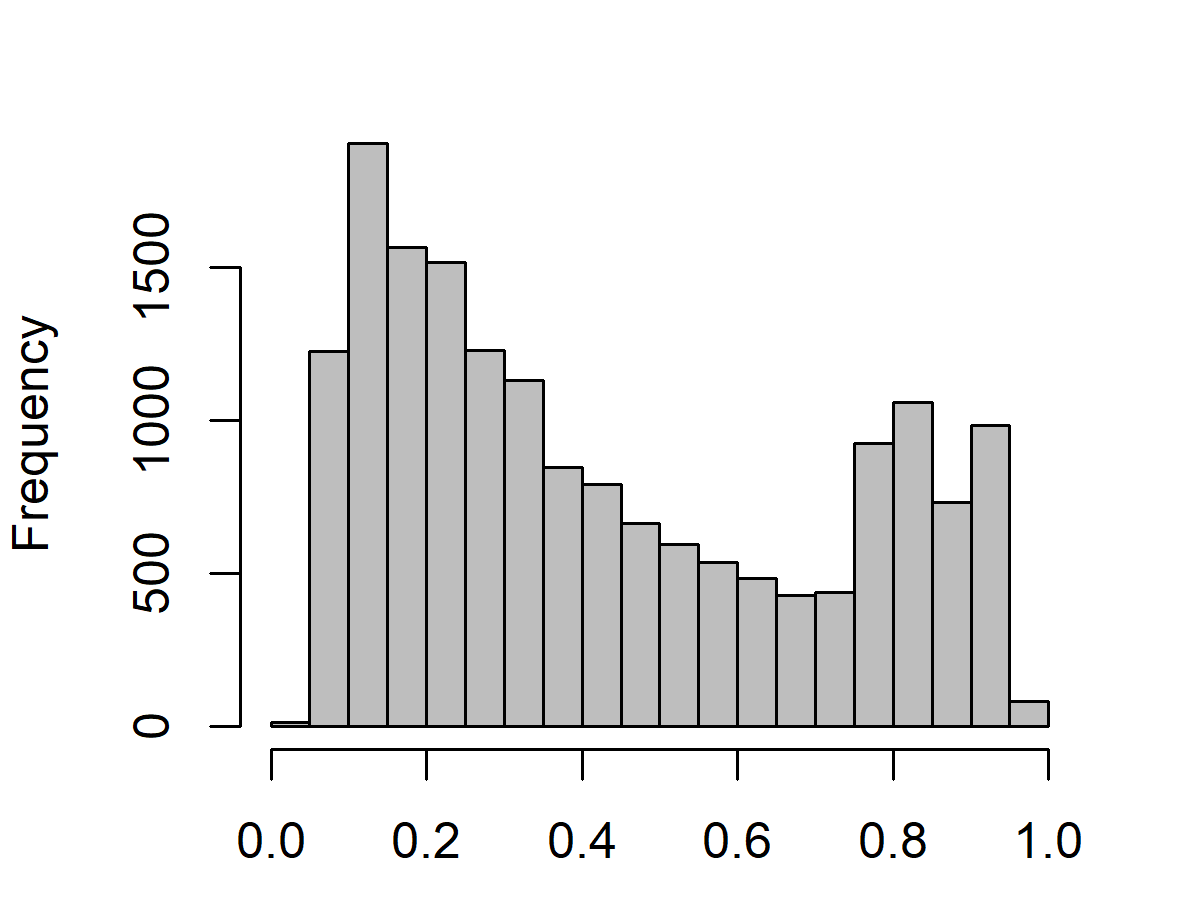
\includegraphics[width=4in]{figures/2SentimentsJST_Histogram.png}
\caption{Histogram of the sentiment scores computed by the Joined Sentiment Topic model}
\label{fig:JSTSentiment}
\end{figure}

The results of the unsupervised Joint Sentiment Models are difficult to evaluate and we have to be at least wary of the results we obtained. Problematic in this case could also be, that the JST views the documents as bag of words and therefore also ignores the ordering of words. Business language contains a lot of fixed phrases that are not considered here.  Nonetheless they might be an informative feature for the estimation of stock price movements in the next section. 


\subsection{\textcolor{yellow}{XG-Boost on sentiment data}}\label{sec:XGB}
Based on the RavenPack data and our own custom sentiment scores we tried to make predictions for the movement of the time series of different stocks. Inspired by different Kaggle competitions and \citep{li2018predicting} we decided to try using XGBoost for binary classification of upwards of downwards movement. For continuous predictions, considering the time dependent structure see section ??????. Here the special time dependent structure of the time series is mostly disregarded and instead a gradient tree boosting algorithm called XGBoost will be used. A additional benefit of doing this is the identification if our sentiment scores or the ones from RavenPack are useful in predicting the movement. \\

XGBoost is a gradient tree boosting method developed by \citet{Chen_2016} and has several beneficial properties. Next to the computational properties it scales well for large data sets and can handle missing values internally. A possible competitor would be LightGBM by \citet{Ke2017LightGBMAH} from Microsoft. The general idea behind tree boosting is that they split data it leaf wise with the best fit, whereas other boosting algorithms split the tree level wise. This means splits are done only at the position where the loss can be reduced the most. Each model consists of a predefined number of trees trying to complement each other with a set of classification and regression trees (CART). The tree ensemble method was originally developed by \citet{friedman2001greedy} and XGBoost which stands for \enquote{Extreme Gradient Boosting} can be seen as an extension of the framework. Most of the improvements where done in finding the optimal split at each level, leaf of the tree, because enumerating over all possible solutions is usually computationally impossible. 
% good explanation: https://xgboost.readthedocs.io/en/latest/index.html
% mehr mathe?
%https://homes.cs.washington.edu/~tqchen/2016/03/10/story-and-lessons-behind-the-evolution-of-xgboost.html
For the sentiment data we engineered the different features from the reports. From the sentiment analysis we obtained two scores, one from the simple bag of words method and the other from the JST model. Because there are sometimes multiple reports for one day we took the mean and recorded the standard deviation of the results as well. The number of reports per day was saved in a different variable. As time dependent features we gave the model the log returns of the previous day (logR yest) and today (logR today) as well as the trading volume at that day, see table \ref{tab:predictionFrame}. We are trying to predict if the log returns on the next day are either positive or negative, a binary target. Because we do not have reports for every day the training and testing data only works with the existing days.
From the RavenPack sentiment data we tried all the given variables together with "logR yest", "logR today" and "Volume". The RavenPack data is complete and has records for every day but some days have missing values when there was no sentiment recorded. Missing values are handled internally by XGBoost \citep{Chen_2016}. The model learns automatically where to go when a value is missing. For a large enough amount of data this is similar to imputing a value but based on a reduction on training loss. This i a benefit of XGBoost. 
\begin{table}[h]
\centering
\begin{tabular}{lrrrrrrr}
\toprule
{} &  logR today &  Volume &  logR yest. &  sent1 &  sentBoW &  sent1 sd &  \dots \\
utc\_date   &              &             &                     &             &               &           &                   \\
\midrule
2012-01-03 &       0.0000 &  45M &           0.0000 &      0.2790 &       -0.6190 &    0.0000 &         \dots \\
2012-01-04 &       0.0230 &  48M &              0.0000 &      0.7019 &        0.2318 &    0.1843 &      \dots \\
2012-01-05 &       0.0116 &  49M &              0.0230 &      0.1413 &        0.0000 &    0.0069 &      \dots \\
2012-01-06 &      -0.0060 &  36M &              0.0116 &      0.4749 &        0.1205 &    0.0257 &      \dots\\
2012-01-09 &       0.0090 &  47M &             -0.0060 &      0.6006 &       -0.6842 &    0.4526 &      \dots \\
2012-01-11 &       0.0084 &  57M &              0.0090 &      0.3607 &       -0.0296 &    0.2511 &      \dots \\
2012-01-12 &      -0.0020 &  44M &              0.0084 &      0.4279 &        0.0668 &    0.1181 &      \dots \\
2012-01-13 &      -0.0239 &  63M &             -0.0020 &      0.4603 &       -0.0076 &    0.2330 &      \dots \\
\bottomrule
\end{tabular}
    \label{tab:predictionFrame}
    \caption{Excerpt from the data frame used for predictions}
\end{table} 
The data was split into a training, validation and testing split by cutting the time series a predefined dates. Around 80 Percent where used for training and validation and testing is done out of sample on values after 2016-12-10. For each stock an independent model was fit and refitted after each prediction. After testing different hyper parameters we settled on a specification with 200 trees, a maximum depth of three, a learning rate of 0.05 and $\eta = 0.1$. Figure \ref{fig:tree} displays a random tree from the XGBoost tree ensemble for the RavenPack sentiment data. \\ 
%\begin{figure}[h]
%\centering
%\includegraphics[width=\textwidth]{figures/treeRavenpack.png}
%\caption{Random tree from the RavenPack tree ensemble}
%\label{fig:tree}
%\end{figure}

Even though we tried different hyper parameters none seemed to make a large difference. Prediction accuracy was always around 50 Percent and the F1-measure (\ref{eq:f1score}) a standard evaluation metric of binary classification results \citep{HADDI201326} was consistently below 0.5.
\begin{equation} 
    F-measure = \frac{2*precision * recall}{precision + recall}
\end{equation}\label{eq:f1score}
The results for the RavenPack data and our own sentiment scores can be found in Table \ref{tab:RavSentRes} and \ref{tab:OurSentRes}. By looking at the cross tables we also discovered that for some stocks class imbalances might cause the algorithm to mostly predict one class. 
\begin{table}[h]
\centering
\begin{tabular}{lrrrr}
\toprule
{} &  f1\_score &  accuracy &  precision &    recall \\
ticker &           &           &            &           \\
\midrule
MMM    &  0.360465 &  0.584906 &   0.574074 &  0.262712 \\
AXP    &  0.410000 &  0.554717 &   0.506173 &  0.344538 \\
GE     &  0.593272 &  0.498113 &   0.557471 &  0.633987 \\
INTC   &  0.452991 &  0.516981 &   0.456897 &  0.449153 \\
JNJ    &  0.413146 &  0.528302 &   0.543210 &  0.333333 \\
PG     &  0.520147 &  0.505660 &   0.493056 &  0.550388 \\
UTX    &  0.323699 &  0.558491 &   0.509091 &  0.237288 \\
VZ     &  0.479087 &  0.483019 &   0.504000 &  0.456522 \\
V      &  0.454936 &  0.513410 &   0.430894 &  0.481818 \\
DIS    &  0.331707 &  0.483019 &   0.478873 &  0.253731 \\
\bottomrule
\end{tabular}
    \label{tab:RavSentRes}
    \caption{Prediction results for RavenPack sentiment data using XGBoost binary classification}
\end{table}
%
\begin{table}[h]
\centering
\begin{tabular}{lrrrr}
\toprule
{} &  f1\_score &  accuracy &  precision &    recall \\
ticker &           &           &            &           \\
\midrule
MMM    &  0.2745 &  0.4788 &   0.4666 &  0.1944 \\
AXP    &  0.5263 &  0.4943 &   0.4385 &  0.6578 \\
GE     &  0.4836 &  0.4513 &   0.5606 &  0.4252 \\
INTC   &  0.3055 &  0.5575 &   0.3548 &  0.2682 \\
JNJ    &  0.2380 &  0.5362 &   0.4347 &  0.1639 \\
PG     &  0.4556 &  0.4487 &   0.4864 &  0.4285 \\
UTX    &  0.4556 &  0.4342 &   0.4000 &  0.5294 \\
VZ     &  0.4742 &  0.5142 &   0.5476 &  0.4181 \\
V      &  0.3437 &  0.4683 &   0.3548 &  0.3333 \\
DIS    &  0.4948 &  0.5663 &   0.6486 &  0.4000 \\
\bottomrule
\end{tabular}
    \label{tab:OurSentRes}
    \caption{Prediction results for analyst reports sentiments using XGBoost binary classification}
\end{table}
Variable importance plots can help to identify how important certain features are for the trees. In figure \ref{fig:VIP} the feature importance for the RavenPack data is displayed on the left and the importance for the sentiment scores is on the right. For the RavenPack data the estimated novelty score loads the highest followed by the number of events over a 90 day period. For the sentiment data from the analyst reports trading volume and the two sentiment scores contain the most information according to the model. Over the course of trying different model specifications the sentiment score from the library method reliably outperformed the Joint Sentiment Topic model. The standard deviation of the JST sentiment scores seemed to hold no meaning for the model. These visual results need to be treated with care, because the model precision appears to be relatively poor. Looking at the classification error and log loss the models did not seem to converge properly. This is a classical downside of gradient tree boosting methods as many statistical convergence measures are not applicable. It would also be interesting to obtain a probability of the certain movement instead of only the binary classification. Our results are similar to the ones by \citet{atkins2018financial} in that our prediction accuracy is usually lower than 50 Percent. 
\begin{figure}[h!]
    \centering
    \figuretitle{Feature Importance Plots}
    \begin{adjustbox}{width=.95\textwidth,center}
        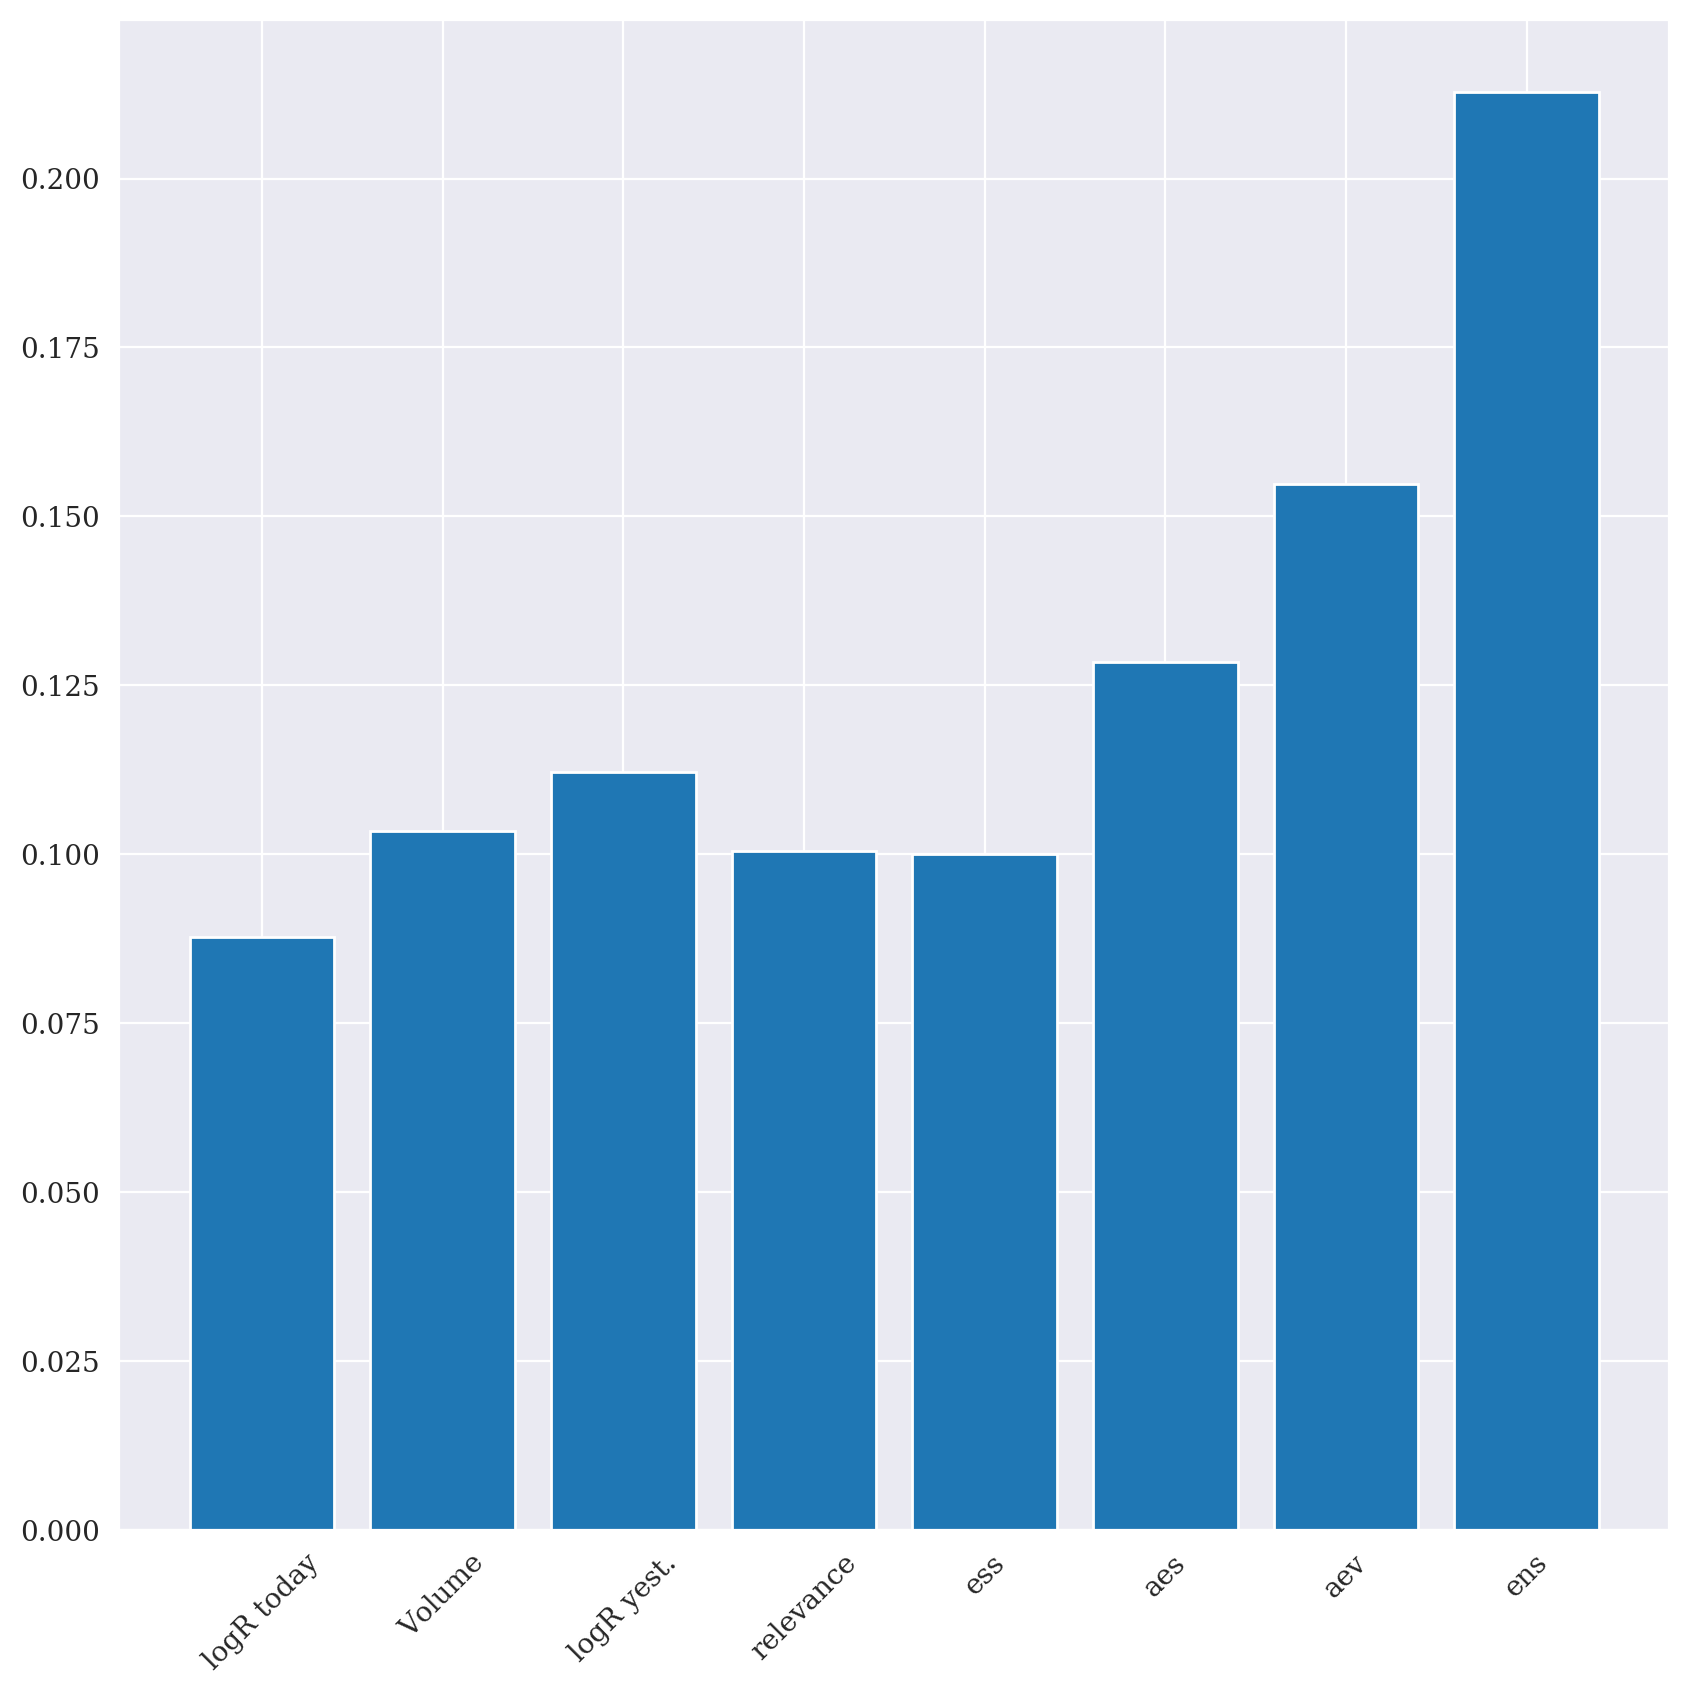
\includegraphics[width = \linewidth]{figures/XGBoostRav_tomorrow_iterative.png}
        %\input{figures/XGBoostRav_tomorrow_iterative.png}
        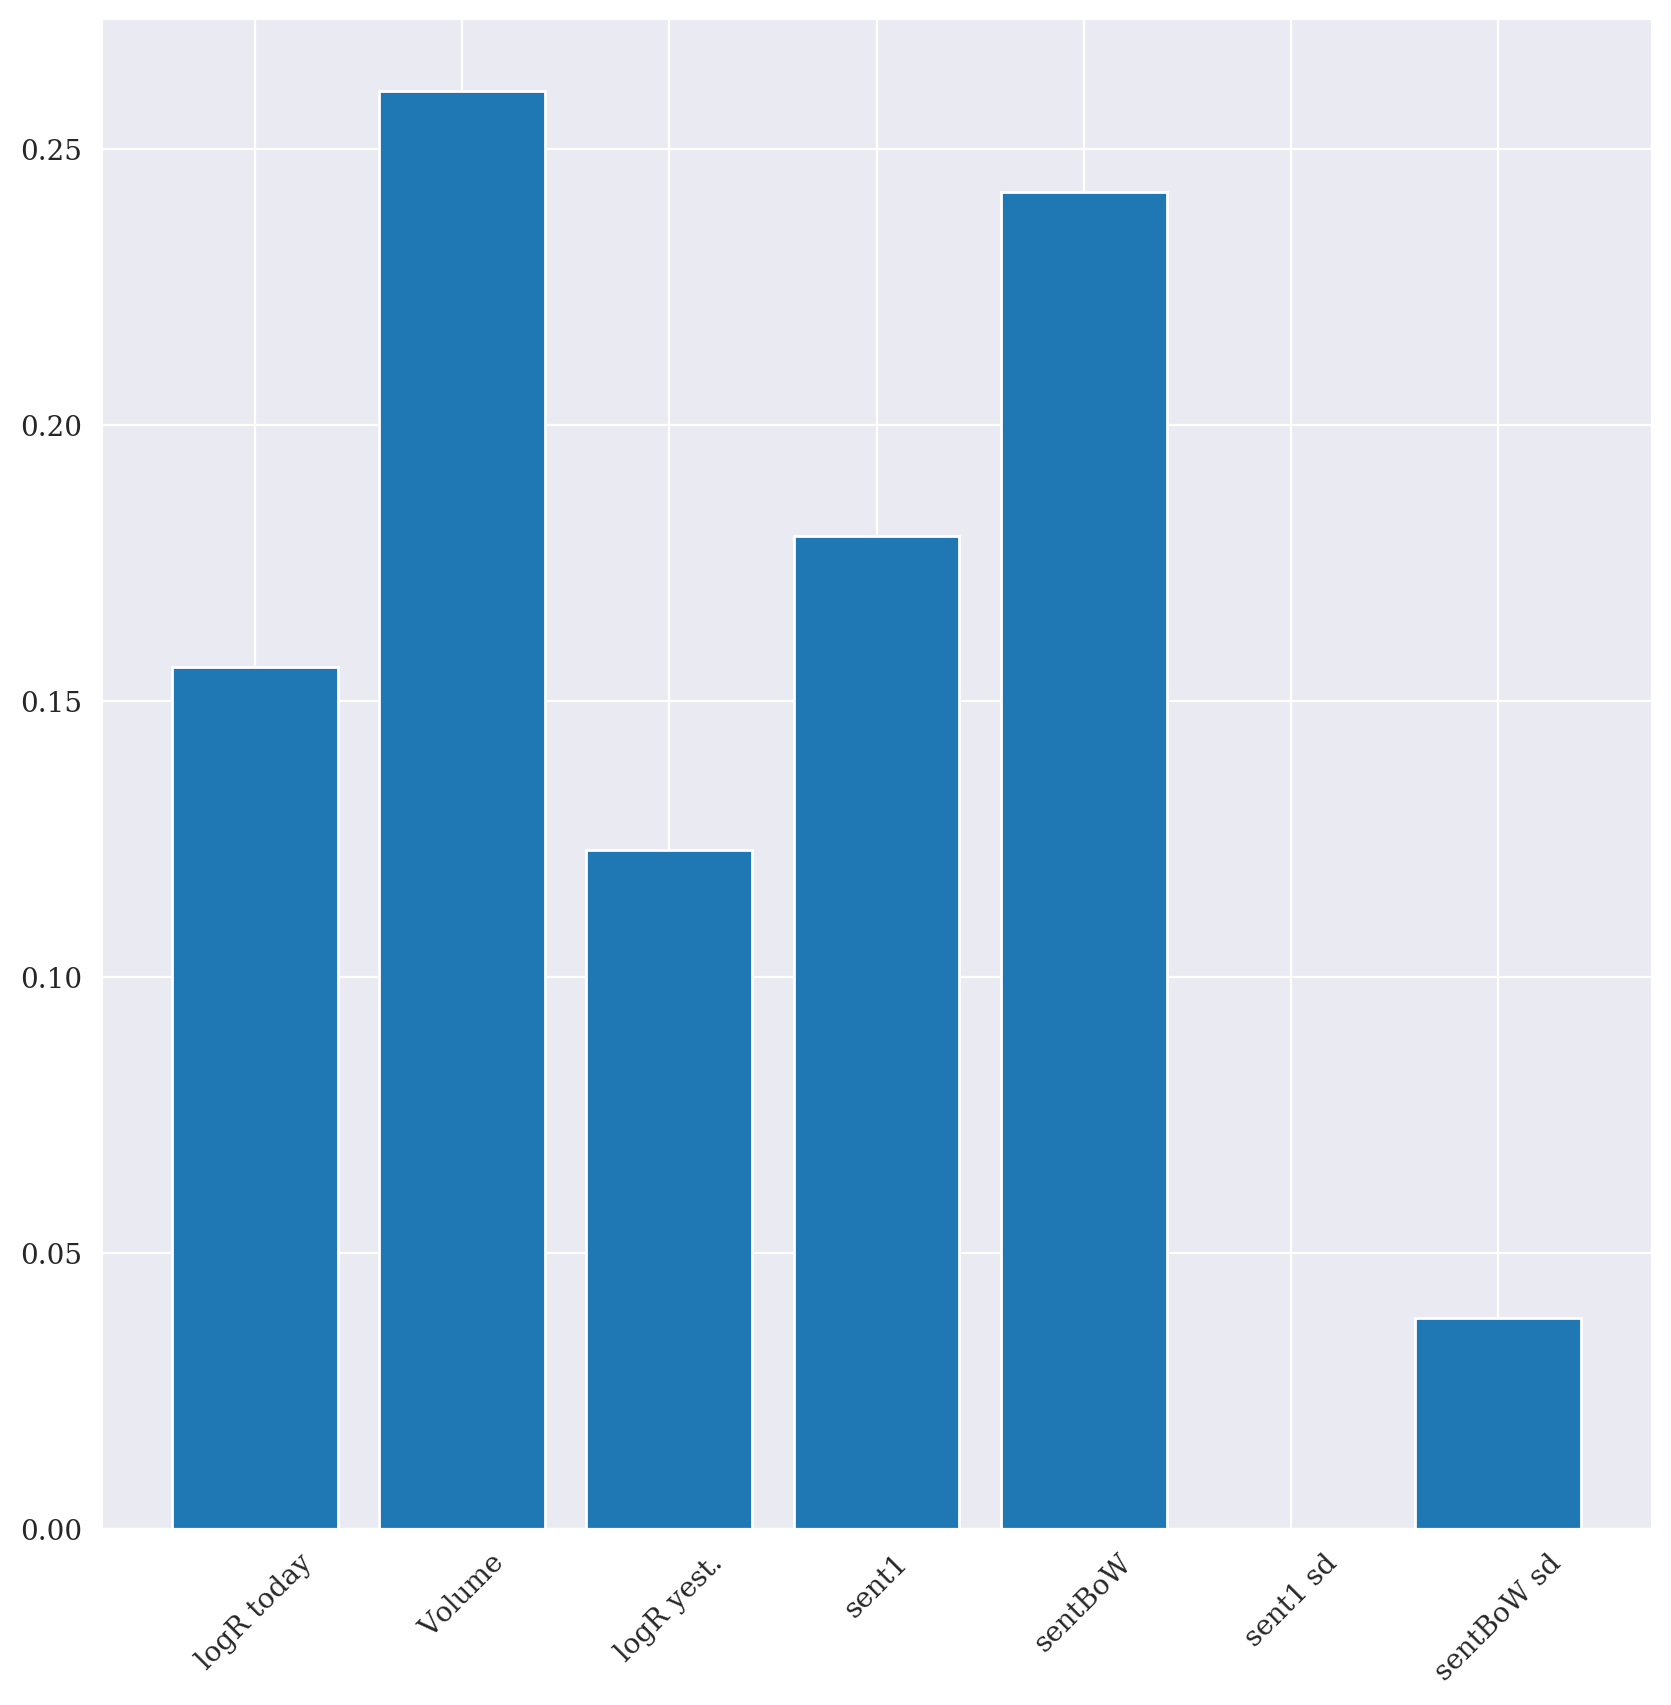
\includegraphics[width = \linewidth]{figures/XGBoostSent_tomorrow_iterative.png}
        %\input{figures/XGBoostSent_tomorrow_iterative.png}
    \end{adjustbox}  
    \caption{On the left the feature importance plot for RavenPack model and on the right the corresponding one for the analyst reports.}
    \label{fig:VIP}
\end{figure}
%What would have also be interesting would be to model market uncertainty and volatility as opposed to the movement of the time series itself. 



